\chapter{Probabilité conditionnelle}

\section{Notions fondamentales de probabilité}

\subsection{Définition et propriétés}

\begin{defin}
	Dans le cadre de l'étude des probabilités :

	\begin{itemize}
		\item Une \textbf{expérience aléatoire} est une épreuve dont le résultat dépend du hasard et ne peut pas être prédit avec certitude avant qu'elle ne soit réalisée.
		\item Une \textbf{issue} est un résultat possible de l'expérience aléatoire.
		\item L'\textbf{univers}, noté $\Omega$, est l'ensemble de toutes les issues possibles de cette expérience.
		\item Un \textbf{événement} est une partie de l'univers, c'est-à-dire un ensemble constitué d'une ou de plusieurs issues.
	\end{itemize}
\end{defin}

\begin{exemple}
	On lance un dé équilibré à 6 faces :

	\begin{itemize}
		\item L'\textbf{expérience aléatoire} est le lancer du dé.
		\item Une \textbf{issue} est l'obtention d'un nombre (par exemple, le $\epsdice{3}$).
		\item L'\textbf{univers} est l'ensemble de tous les résultats possibles : $\Omega = \brac{\epsdice{1}\,;\,\epsdice{2}\,;\,\epsdice{3}\,;\,\epsdice{4}\,;\,\epsdice{5}\,;\,\epsdice{6}}$.
		\item Un \textbf{événement} est par exemple $A$ : \og obtenir un nombre pair \fg{}, ce qui correspond à la partie $\brac{\epsdice{2}\,;\,\epsdice{4}\,;\,\epsdice{6}}$.
	\end{itemize}
\end{exemple}

\begin{defin}
	La \textbf{probabilité d'une issue} correspond à la fréquence à laquelle cette issue se réalise si on répète l'expérience aléatoire un très grand nombre de fois (fréquence stabilisée à long terme).
\end{defin}

\begin{ex}
	Si on choisit une personne au hasard en France, la proportion de gauchers étant estimée à $14\,\%$, la probabilité de choisir une personne gauchère est de $0,14$.
\end{ex}

\begin{ex}
	On considère une classe de $30$ élèves comprenant $18$ filles et $12$ garçons. On choisit un élève au hasard.

	L'univers de cette expérience aléatoire est $\Omega = \{\text{Fille}, \text{Garçon}\}$.

	Les deux issues ne sont pas équiprobables :

	\begin{itemize}
		\item La probabilité de l'issue \og Fille\fg{} est : $\p{\text{Fille}} = \dfrac{18}{30} = \dfrac{3}{5} = 0{,}6$
		\item La probabilité de l'issue \og Garçon\fg{} est : $\p{\text{Garçon}} = \dfrac{12}{30} = \dfrac{2}{5} = 0{,}4$
	\end{itemize}
\end{ex}

\begin{defin}
	Soit une expérience aléatoire dont l'univers est $\Omega = \{e_1, e_2, \dots, e_n\}$.

	Définir une \textbf{loi de probabilité}, c'est associer à chaque issue $e_i$ un nombre réel $p_i$, appelé probabilité de l'issue, tel que :

	\begin{itemize}
		\item $0 \leqslant p_i \leqslant 1$ pour chaque issue $e_i$ ;
		\item La somme de toutes les probabilités est égale à $1$ : $\quad p_1 + p_2 + \dots + p_n = 1$.
	\end{itemize}
\end{defin}

\newpage

\begin{rem}
	Cette loi est généralement présentée sous la forme d'un tableau :

	\begin{center}
		\rnc{\arraystretch}{1.3}
		\begin{tabular}{|c|c|c|c|c|} \hline
			\textbf{Issue} $e_i$       & $e_1$ & $e_2$ & $\dots$ & $e_n$ \\ \hline
			\textbf{Probabilité} $p_i$ & $p_1$ & $p_2$ & $\dots$ & $p_n$ \\ \hline
		\end{tabular}
	\end{center}
\end{rem}

\begin{ex}
	Reprenons l'exemple de la classe composée de $18$ filles et $12$ garçons ($30$ élèves en tout).

	Si on choisit un élève au hasard, la loi de probabilité associée à cette expérience est donnée par le tableau suivant :

	\begin{center}
		\rnc{\arraystretch}{1.5}
		\begin{tabular}{|c|c|c|} \hline
			\textbf{Issue} $e_i$       & Fille                   & Garçon                  \\ \hline
			\textbf{Probabilité} $p_i$ & $\frac{18}{30} = 0{,}6$ & $\frac{12}{30} = 0{,}4$ \\ \hline
		\end{tabular}
	\end{center}

	On vérifie bien que la somme des probabilités est égale à $1$ : $0{,}6 + 0{,}4 = 1$.
\end{ex}

\begin{prop}
	Soit $A$ un événement d'une expérience aléatoire.

	Si $A$ est constitué des issues $e_1, e_2, \dots, e_k$, alors la probabilité de l'événement $A$ est donnée par :
	\[
		\p{A} = \p{e_1} + \p{e_2} + \dots + \p{e_k}
	\]

	C'est-à-dire que la probabilité d'un événement est la somme des probabilités des issues qui le réalisent.
\end{prop}

\begin{rem}
	Par convention, la probabilité de l'événement impossible, noté $\emptyset$, est égale à $0$.
\end{rem}

\begin{prop}
	Soit une expérience aléatoire définie sur un univers $\Omega = \{e_1, e_2, \dots, e_n\}$ dont la loi de probabilité est donnée par le tableau suivant :

	\begin{center}
		\rnc{\arraystretch}{1.3}
		\begin{tabular}{|c|c|c|c|c|} \hline
			\textbf{Issue} $e_i$       & $e_1$ & $e_2$ & $\dots$ & $e_n$ \\ \hline
			\textbf{Probabilité} $p_i$ & $p_1$ & $p_2$ & $\dots$ & $p_n$ \\ \hline
		\end{tabular}
	\end{center}

	\begin{itemize}
		\item La somme des probabilités de toutes les issues est toujours égale à $1$ :
		      \[
			      p_1 + p_2 + \dots + p_n = \p{\Omega} = 1
		      \]

		\item La probabilité de l'événement contraire $\bar{A}$ se calcule par :
		      \[
			      \quad \p{\bar{A}} = 1 - \p{A}
		      \]
	\end{itemize}
\end{prop}

\begin{ex}
	\nline

	\begin{itemize}
		\item \textbf{Expérience aléatoire :} Lancer un dé à 6 faces.
		\item \textbf{Univers :} $\Omega = \left\{\epsdice{1}\,;\,\epsdice{2}\,;\,\epsdice{3}\,;\,\epsdice{4}\,;\,\epsdice{5}\,;\,\epsdice{6}\right\}$
		\item \textbf{Événement $E$ :} \og{} On obtient un nombre pair \fg{}
		      \[
			      E = \left\{\epsdice{2}\,;\,\epsdice{4}\,;\,\epsdice{6}\right\}
		      \]
		\item \textbf{Calcul de probabilité :}
		      \[
			      \p{E} = \p{\epsdice{2}} + \p{\epsdice{4}} + \p{\epsdice{6}} = \dfrac{3}{6} = 0{,}5
		      \]
		\item \textbf{Événement contraire $\bar{E}$ :} \og{} Obtenir un nombre impair \fg{}
		      \[
			      \p{\bar{E}} = 1 - \p{E} = 1 - 0{,}5 = 0{,}5
		      \]
	\end{itemize}
\end{ex}

\subsection{Intersection et union d'événements}

\begin{prop}
	Soient $A$ et $B$ deux événements d'une même expérience aléatoire.

	\begin{itemize}
		\item \textbf{Intersection ($A \cap B$) :}

		      L'événement \og{} $A \text{ et } B$ \fg{}, noté $A \cap B$, est constitué de toutes les issues qui réalisent \textbf{à la fois} l'événement $A$ \textbf{et} l'événement $B$.

		\item \textbf{Union ($A \cup B$) :}

		      L'événement \og{} $A \text{ ou } B$ \fg{}, noté $A \cup B$, est constitué de toutes les issues qui réalisent l'événement $A$, l'événement $B$, \textbf{ou les deux en même temps}.
	\end{itemize}
\end{prop}

\begin{ex}
	On considère l'expérience aléatoire qui consiste à lancer un dé à 6 faces, dont l'univers est noté $\Omega$.

	On a :
	\[
		\Omega = \left\{\epsdice{1}\,;\,\epsdice{2}\,;\,\epsdice{3}\,;\,\epsdice{4}\,;\,\epsdice{5}\,;\,\epsdice{6}\right\}
	\]

	Soit les événements :

	\begin{itemize}
		\item $E$ : \og{} Obtenir un nombre pair \fg{} $\quad\Rarr E = \left\{\epsdice{2}\,;\,\epsdice{4}\,;\,\epsdice{6}\right\}$
		\item $F$ : \og{} Obtenir au plus $4$ \fg{} $\quad\Rarr F = \left\{\epsdice{1}\,;\,\epsdice{2}\,;\,\epsdice{3}\,;\,\epsdice{4}\right\}$
	\end{itemize}

	\begin{enumerate}
		\item \textbf{Intersection d'événements (\og{} ET \fg{})}

		      Soit $G$ l'événement : \og{} Obtenir un nombre pair \textbf{et} au plus $4$ \fg{}.

		      On a $G = E \text{ et } F$, noté plus simplement $G = E \cap F$.

		      Les issues réalisant à la fois $E$ et $F$ sont $\epsdice{2}$ et $\epsdice{4}$, donc $G = \left\{\epsdice{2}\,;\,\epsdice{4}\right\}$.
		      \[
			      \p{G} = \p{E \cap F} = \p{\epsdice{2}} + \p{\epsdice{4}} = \dfrac{2}{6} = \dfrac{1}{3}
		      \]

		\item \textbf{Union d'événements (\og{} OU \fg{})}

		      Soit $H$ l'événement : \og{} Obtenir un nombre pair \textbf{ou} au plus $4$ \fg{}.

		      On a $H = E \text{ ou } F$, noté $H = E \cup F$.

		      Cet événement rassemble toutes les issues qui réalisent $E$, $F$, ou les deux, donc $H = \left\{\epsdice{1}\,;\,\epsdice{2}\,;\,\epsdice{3}\,;\,\epsdice{4}\,;\,\epsdice{6}\right\}$.
		      \[
			      \def\arraystretch{1.5}
			      \begin{array}{rcl}
				      \p{H} & = & \p{E \cup F}                                                                            \\
				            & = & \p{\epsdice{1}} + \p{\epsdice{2}} + \p{\epsdice{3}} + \p{\epsdice{4}} + \p{\epsdice{6}} \\
				            & = & \dfrac{5}{6} \approx 0{,}833
			      \end{array}
		      \]
	\end{enumerate}
\end{ex}

\begin{prop}
	Soient $A$ et $B$ deux événements d'une même expérience aléatoire. Pour tous événements $A$ et $B$, on a la relation : \[
		\p{A \cup B} = \p{A} + \p{B} - \p{A \cap B}
	\]

\end{prop}

\begin{ex}
	\nline
	\begin{wrapstuff}[r]
		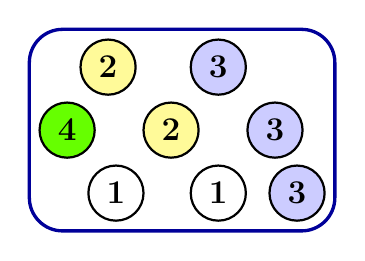
\begin{tikzpicture}[scale=0.4,
				ball/.style={circle, draw=black, thick, text=black, font=\bfseries\large, minimum size=0.7cm, inner sep=0pt},
				ball1/.style={ball, fill=white},
				ball2/.style={ball, fill=yellow!40},
				ball3/.style={ball, fill=blue!20},
				ball4/.style={ball, fill=green!60!yellow}
			]
			\draw[blue!60!black, very thick, rounded corners=12pt] (-1, -0.7) rectangle (8.7, 5.7);
			\node[ball2] at (1.5, 4.5) {2};
			\node[ball3] at (5.0, 4.5) {3};
			\node[ball4] at (0.2, 2.5) {4};
			\node[ball2] at (3.5, 2.5) {2};
			\node[ball3] at (6.8, 2.5) {3};
			\node[ball1] at (1.75, 0.5) {1};
			\node[ball1] at (5.0, 0.5) {1};
			\node[ball3] at (7.5, 0.5) {3};
		\end{tikzpicture}
	\end{wrapstuff}
	On tire une boule dans l'urne ci-contre.

	On a :
	\[
		\Omega=\left\{1\,;\,2\,;\,3\,;\,4\right\}
	\]

	On définit les événements suivants :

	\begin{itemize}
		\item $A$ : \og{} Tirer une boule portant le numéro $1$ ou $2$ \fg{} $\quad\Rarr A = \{1\,;\,2\}$
		\item $C$ : \og{} Tirer une boule portant le numéro $1$ ou $3$ \fg{} $\quad\Rarr C = \{1\,;\,3\}$
	\end{itemize}

	\newpage

	\textbf{Calculs de probabilités et relations :}

	\begin{itemize}
		\item \textbf{Probabilité de $A$ et $C$ :}
		      \[
			      \p{A} = \dfrac{4}{8} = 0{,}5 \quad\text{et}\quad \p{C} = \dfrac{5}{8} = 0{,}625
		      \]
		\item \textbf{Événement contraire $\bar{A}$ :} \og{} Ne pas être dans $A$ \fg{}
		      \[
			      \bar{A} = \{3\,;\,4\} \quad\text{donc}\quad \p{\bar{A}} = \dfrac{4}{8} = 0{,}5
		      \]
		\item \textbf{Intersection $A \cap C$ :} \og{} Être à la fois dans $A$ et dans $C$ \fg{}
		      \[
			      A \cap C = \{1\} \quad\text{donc}\quad \p{A \cap C} = \dfrac{2}{8} = 0{,}25
		      \]
		\item \textbf{Union $A \cup C$ :} \og{} Être dans $A$ ou dans $C$ \fg{}
		      \[
			      A \cup C = \{1\,;\,2\,;\,3\} \quad\text{donc}\quad \p{A \cup C} = \dfrac{7}{8} = 0{,}875
		      \]
		\item \textbf{Diagramme de Venn}
		      \begin{center}
			      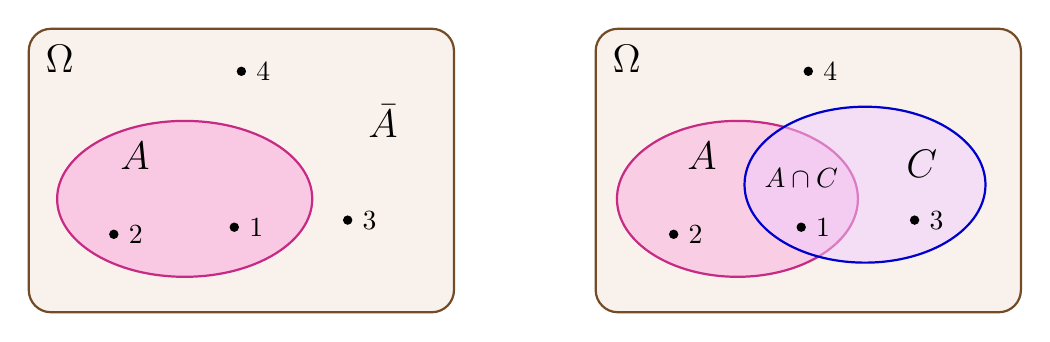
\begin{tikzpicture}[scale=0.9, dot/.style={circle, fill=black, inner sep=1.2pt} ]
				      \begin{scope}[shift={(0,0)}]
					      \draw[brown!60!black, thick, fill=brown!10, rounded corners=8pt] (0,0) rectangle (6,4);
					      \node[anchor=north west] at (0.1, 3.9) {\Large $\Omega$};
					      \draw[magenta!80!black, thick, fill=magenta!25, fill opacity=0.8] (2.2, 1.6) ellipse (1.8cm and 1.1cm);
					      \node at (1.5, 2.2) {\Large $A$};
					      \node at (5.0, 2.7) {\Large $\bar{A}$};
					      \node[dot, label=right:{$1$}] at (2.9, 1.2) {};
					      \node[dot, label=right:{$2$}] at (1.2, 1.1) {};
					      \node[dot, label=right:{$3$}] at (4.5, 1.3) {};
					      \node[dot, label=right:{$4$}] at (3.0, 3.4) {};
				      \end{scope}
				      \begin{scope}[shift={(8,0)}]
					      \draw[brown!60!black, thick, fill=brown!10, rounded corners=8pt] (0,0) rectangle (6,4);
					      \node[anchor=north west] at (0.1, 3.9) {\Large $\Omega$};
					      \draw[magenta!80!black, thick, fill=magenta!25, fill opacity=0.7] (2.0, 1.6) ellipse (1.7cm and 1.1cm);
					      \draw[blue!80!black, thick, fill=blue!30!magenta!20, fill opacity=0.5] (3.8, 1.8) ellipse (1.7cm and 1.1cm);
					      \node at (1.5, 2.2) {\Large $A$};
					      \node at (4.6, 2.1) {\Large $C$};
					      \node at (2.9, 1.9) {$A \cap C$};
					      \node[dot, label=right:{$1$}] at (2.9, 1.2) {};
					      \node[dot, label=right:{$2$}] at (1.1, 1.1) {};
					      \node[dot, label=right:{$3$}] at (4.5, 1.3) {};
					      \node[dot, label=right:{$4$}] at (3.0, 3.4) {};
				      \end{scope}
			      \end{tikzpicture}
		      \end{center}
	\end{itemize}
\end{ex}

\section{Probabilité conditionnelle}

\subsection{Définition}

\begin{defin}
	Dans une population ou un ensemble réparti selon deux critères :

	\begin{itemize}
		\item Une \textbf{fréquence marginale} correspond au rapport entre l'effectif d'une sous-population totale (considérant un seul critère) et l'effectif total de l'étude.
		\item Une \textbf{fréquence conditionnelle} correspond au rapport entre l'effectif d'une sous-population satisfaisant à la fois plusieurs critères et l'effectif restreint à une condition particulière.
	\end{itemize}
\end{defin}

\begin{ex}
	Sur un groupe de $100$ élèves, $40$ sont des filles et $15$ filles jouent au tennis.

	\begin{itemize}
		\item La \textbf{fréquence marginale} des filles est $\dfrac{40}{100} = 0{,}4$.
		\item La \textbf{fréquence conditionnelle} des joueuses de tennis parmi les filles est $\dfrac{15}{40} = 0{,}375$.
	\end{itemize}
\end{ex}

\newpage

\subsection{Calcul à l'aide d'un tableau croisé}

\begin{methode}[Déterminer une fréquence conditionnelle / marginale]
	Dans une entreprise qui compte $360$ employés, on compte :

	\begin{itemize}
		\item $60\%$ d'hommes et parmi ceux-là, $12,5 \%$ sont des cadres.
		\item Par ailleurs, $87,5\%$ des femmes de cette entreprise sont ouvrières ou techniciennes.
	\end{itemize}

	\begin{enumerate}
		\item Modéliser la situation à l'aide d'un tableau d'effectifs.
		\item Calculer la fréquence marginale des cadres.
		\item Calculer la fréquence conditionnelle des ouvriers et techniciens parmi les hommes.
	\end{enumerate}

	\begin{correction}
		\nline
		\begin{enumerate}
			\item Avec l'énoncé, le tableau d'effectif est le suivant :
			      \begin{center}
				      \rnc{\arraystretch}{1.3}
				      \begin{tabular}{|c|c|c|c|}
					      \hline
					      ~                   & \ccg{Hommes}          & \ccg{Femmes}           & \ccg\textbf{Total} \\ \hline
					      \ccg {Cadres}       & $12,5\%\times 216=27$ & $144-126=18$           & $27+18=45$         \\ \hline
					      \ccg {Ouvriers}     & $216-27=189$          & $87,5\%\times 144=126$ & $189+126=315$      \\ \hline
					      \ccg \textbf{Total} & $60\%\times 360=216$  & $360-216=144$          & $360$              \\ \hline
				      \end{tabular}
			      \end{center}

			\item La \textbf{fréquence marginale} se lit en {"marge"} du tableau.
			      \begin{center}
				      \rnc{\arraystretch}{1.3}
				      \begin{tabular}{|c|c|c|c|}
					      \hline
					      ~                   & \ccg{Hommes} & \ccg{Femmes} & \ccg\textbf{Total} \\ \hline
					      \ccg {Cadres}       & $27$         & $18$         & ${45}$             \\ \hline
					      \ccg {Ouvriers}     & $189$        & $126$        & $315$              \\ \hline
					      \ccg \textbf{Total} & $216$        & $144$        & ${360}$            \\ \hline
				      \end{tabular}
			      \end{center}

			      On compte $360$ employés en tout et $45$ sont des cadres.

			      La \textbf{fréquence marginale} de cadres est donc égale à :
			      \[
				      \dfrac{45}{360} = 0,125 = 12,5 \%
			      \]

			\item La \textbf{fréquence conditionnelle} restreint l'effectif total.

			      Calculons la fréquence \textbf{conditionnelle d'ouvriers, techniciens} parmi {les hommes}.

			      Ici, on ne considère que les hommes car la "condition" est {"parmi les hommes"}.

			      La \textbf{fréquence conditionnelle} se lit sur \textbf{une ligne ou une colonne intérieure} du tableau.

			      Ici, on ne va donc considérer que la colonne concernant les hommes (condition).

			      \begin{center}
				      \rnc{\arraystretch}{1.3}
				      \begin{tabular}{|c|c|c|c|} \hline
					      ~                   & \ccg{Hommes} & \ccg{Femmes} & \ccg\textbf{Total} \\ \hline
					      \ccg {Cadres}       & $27$         & $18$         & $45$               \\ \hline
					      \ccg {Ouvriers}     & ${189}$      & $126$        & $315$              \\ \hline
					      \ccg \textbf{Total} & ${216}$      & $144$        & $360$              \\ \hline
				      \end{tabular}
			      \end{center}

			      On compte $216$ hommes en tout et parmi eux, $189$ sont des ouvriers, techniciens.

			      La fréquence \textbf{conditionnelle d'ouvriers, techniciens} parmi {les hommes} est :
			      \[
				      \dfrac{189}{216} = 0,875 = 87,5 \%
			      \]
		\end{enumerate}
	\end{correction}
\end{methode}

\newpage

\begin{defin}
	On appelle \textbf{probabilité conditionnelle} de $B$ sachant $A$, la probabilité que l'événement $B$ se réalise \textbf{sachant que} l'événement $A$ est réalisé.

	On la note :
	\[
		\pc{A}{B}
	\]
\end{defin}

\begin{rem}
	\nline
	\begin{center}
		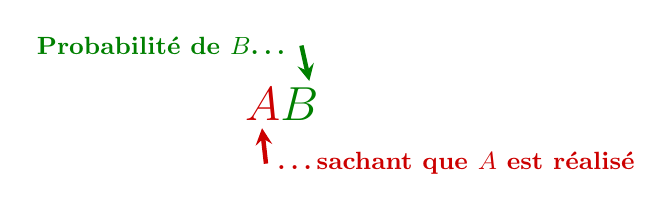
\begin{tikzpicture}[scale=0.5, >=stealth, label_style/.style={font=\small\bfseries, color=blue!80!black} ]
			\node (proba) at (0,0) {\LARGE $\pc{\textcolor{red!80!black}{A}}{\textcolor{green!50!black}{B}}$};
			\draw[<-, ultra thick, green!50!black] (0.7, 0.6) -- (0.5, 1.5) node[left, label_style, color=green!50!black] {Probabilité de $B$\ldots};
			\draw[<-, ultra thick, red!80!black] (-0.5, -0.6) -- (-0.4, -1.5) node[right, label_style, color=red!80!black] {\ldots sachant que $A$ est réalisé};
		\end{tikzpicture}
	\end{center}
\end{rem}

\begin{methode}[Calculer une probabilité conditionnelle à l'aide d'un tableau croisé]
	Dans une classe, la répartition des élèves selon leur genre et la marque de leur téléphone est donnée par le tableau suivant :

	\begin{center}
		\rnc{\arraystretch}{1.3}
		\begin{tabular}{|c|c|c|c|}
			\hline
			~                   & \ccg{Filles} & \ccg{Garçons} & \ccg\textbf{Total} \\ \hline
			\ccg {Apple}        & $10$         & $11$          & $21$               \\ \hline
			\ccg {Samsung}      & $7$          & $2$           & $9$                \\ \hline
			\ccg \textbf{Total} & $17$         & $13$          & $30$               \\ \hline
		\end{tabular}
	\end{center}

	\begin{itemize}
		\item \textbf{Expérience aléatoire :} On choisit un élève au hasard dans la classe.
		\item \textbf{Événements :}
		      \begin{itemize}[label=$\bullet$]
			      \item $A$ : \og{} L'élève a un téléphone \textbf{Apple} \fg{}
			      \item $G$ : \og{} L'élève est un \textbf{garçon} \fg{}
		      \end{itemize}
	\end{itemize}

	\begin{enumerate}

		\item Probabilités simples et d'intersections

		      \begin{itemize}
			      \item $\p{A}$ : Probabilité que l'élève choisi possède un téléphone Apple :
			            \[
				            \p{A} = \dfrac{21}{30} = 0,7
			            \]

			            \begin{center}
				            \rnc{\arraystretch}{1.3}
				            \begin{tabular}{|c|c|c|c|} \hline
					            ~                   & \ccg{Filles} & \ccg{Garçons} & \ccg\textbf{Total} \\ \hline
					            \ccg \textbf{Apple} & $10$         & $11$          & $\boxed{21}$       \\ \hline
					            \ccg {Samsung}      & $7$          & $2$           & $9$                \\ \hline
					            \ccg \textbf{Total} & $17$         & $13$          & $\boxed{30}$       \\ \hline
				            \end{tabular}
			            \end{center}

			      \item $\p{A \cap G}$ : Probabilité que l'élève choisi soit un garçon \textbf{et} possède un téléphone Apple :
			            \[
				            \p{A \cap G} = \dfrac{11}{30}
			            \]

			            \begin{center}
				            \rnc{\arraystretch}{1.3}
				            \begin{tabular}{|c|c|c|c|} \hline
					            ~                   & \ccg{Filles} & \ccg{Garçons} & \ccg\textbf{Total} \\ \hline
					            \ccg \textbf{Apple} & $10$         & $\boxed{11}$  & $21$               \\ \hline
					            \ccg {Samsung}      & $7$          & $2$           & $9$                \\ \hline
					            \ccg \textbf{Total} & $17$         & $13$          & $\boxed{30}$       \\ \hline
				            \end{tabular}
			            \end{center}
		      \end{itemize}

		      \newpage

		\item Probabilités conditionnelles (sachant que)

		      \begin{itemize}
			      \item Calculer la probabilité que l'élève soit un garçon \textbf{sachant qu'}il possède un téléphone Apple.
			            \begin{itemize}[label=$\Rightarrow$]
				            \item \textbf{Notation :} $\pc{A}{G}$ (Probabilité de $G$ sachant $A$).
				            \item \textbf{Calcul :} $\pc{A}{G} = \dfrac{11}{21} \approx 0,5238$
			            \end{itemize}

			            \begin{center}
				            \rnc{\arraystretch}{1.3}
				            \begin{tabular}{|c|c|c|c|} \hline
					            ~                   & \ccg{Filles} & \ccg\textbf{Garçons} & \ccg\textbf{Total} \\ \hline
					            \ccg \textbf{Apple} & $10$         & $\boxed{11}$         & $\boxed{21}$       \\ \hline
					            \ccg {Samsung}      & $7$          & $2$                  & $9$                \\ \hline
					            \ccg \textbf{Total} & $17$         & $13$                 & $30$               \\ \hline
				            \end{tabular}
			            \end{center}

			      \item Calculer la probabilité que l'élève possède un téléphone Apple \textbf{sachant qu'}il s'agit d'une fille.
			            \begin{itemize}[label=$\Rightarrow$]
				            \item \textbf{Notation :} $\pc{\bar{G}}{A}$ (Probabilité de $A$ sachant $\bar{G}$).
				            \item \textbf{Calcul :} $\pc{\bar{G}}{A} = \dfrac{10}{17} \approx 0,5882$
			            \end{itemize}

			            \begin{center}
				            \rnc{\arraystretch}{1.3}
				            \begin{tabular}{|c|c|c|c|} \hline
					            ~                   & \ccg\textbf{Filles} & \ccg{Garçons} & \ccg\textbf{Total} \\ \hline
					            \ccg \textbf{Apple} & $\boxed{10}$        & $11$          & $21$               \\ \hline
					            \ccg {Samsung}      & $7$                 & $2$           & $9$                \\ \hline
					            \ccg \textbf{Total} & $\boxed{17}$        & $13$          & $30$               \\ \hline
				            \end{tabular}
			            \end{center}
		      \end{itemize}

		\item Calcul de $\pc{\bar{A}}{\bar{G}}$

		      C'est la probabilité de $\bar{G}$ sachant que $\bar{A}$ est réalisé.
		      \[
			      \pc{\bar{A}}{\bar{G}}=\dfrac{7}{9}\approx 0,777
		      \]

		      \textbf{Parmi} les élèves qui n'ont pas de téléphone Apple, $77,7\%$ élèves sont des filles.

		      \begin{center}
			      \rnc{\arraystretch}{1.3}
			      \begin{tabular}{|c|c|c|c|} \hline
				      ~                     & \ccg\textbf{Filles} & \ccg{Garçons} & \ccg\textbf{Total} \\ \hline
				      \ccg {Apple}          & $10$                & $11$          & $21$               \\ \hline
				      \ccg \textbf{Samsung} & $\boxed{7}$         & $2$           & $\boxed{9}$        \\ \hline
				      \ccg \textbf{Total}   & $17$                & $13$          & $30$               \\ \hline
			      \end{tabular}
		      \end{center}

	\end{enumerate}
\end{methode}

\subsection{Calcul à l'aide de la formule}

\begin{rem}
	On note $\card{A}$ le nombre d'issues de l'événement $A$.
\end{rem}

\begin{prop}
	Les effectifs conjoints et marginaux associés à deux événements $A$ et $B$ se résument dans le tableau croisé suivant :

	\begin{center}
		\rnc{\arraystretch}{1.3}
		\begin{tabular}{|c|c|c|c|} \hline
			~                   & \ccg $B$                & \ccg $\bar{B}$                & \ccg \textbf{Total} \\ \hline
			\ccg $A$            & $\card{A \cap B}$       & $\card{A \cap \bar{B}}$       & $\card{A}$          \\ \hline
			\ccg $\bar{A}$      & $\card{\bar{A} \cap B}$ & $\card{\bar{A} \cap \bar{B}}$ & $\card{\bar{A}}$    \\ \hline
			\ccg \textbf{Total} & $\card{B}$              & $\card{\bar{B}}$              & $\card{\Omega}$     \\ \hline
		\end{tabular}
	\end{center}
\end{prop}

\newpage

\begin{prop}
	Soient $A$ et $B$ deux événements d'une expérience aléatoire, avec $\p{A} \neq 0$.

	La \textbf{probabilité conditionnelle} de l'événement $B$ sachant que l'événement $A$ est réalisé est donnée par :

	\[
		{\pc{A}{B} = \dfrac{\p{A \cap B}}{\p{A}}}
	\]

	Dans le cas où les issues de l'expérience sont \textbf{équiprobables}, cette formule s'exprime à l'aide des effectifs :

	\[
		{\pc{A}{B} = \dfrac{\card{A \cap B}}{\card{A}}}
	\]

\end{prop}

\begin{rem}
	\nline
	\begin{center}
		\begin{tikzpicture}[>=Stealth,scale=0.8]
			\node[font=\LARGE,scale=0.8] at (0,0) {$\pc{A}{B}=\dfrac{\p{A\cap B}}{\p{A}}$};
			\draw[->, ultra thick] (-1.7,-0.4) to[in=-120, out=-70] (1.2,-0.7);
			\draw[ultra thick,looseness=2] (-1.6,0.3) to[in=90, out=90] (-1.1,0.3);
			\draw[->, ultra thick] (-1.35,0.6) to[in=120, out=70] (1.2,0.7);
		\end{tikzpicture}
	\end{center}
\end{rem}

\begin{ex}[Étude pharmaceutique]
	Une étude pharmaceutique est réalisée sur un échantillon de $800$ patients afin d'évaluer l'efficacité de deux nouveaux traitements.

	Au cours de cet essai, les patients ont reçu soit le médicament A, soit le médicament B.

	L'objectif est d'observer l'issue du traitement, en comptabilisant le nombre de personnes guéries et non guéries pour chacun des deux médicaments.

	Les résultats de cette étude sont résumés dans le tableau croisé ci-dessous :

	\begin{center}
		\rnc{\arraystretch}{1.3}
		\begin{tabular}{|c|c|c|c|}
			\hline
			~                  & \ccg{Médicament A} & \ccg{Médicament B} & \ccg\textbf{Total} \\ \hline
			\ccg{Guéri}        & $383$              & $291$              & $674$              \\ \hline
			\ccg{Non guéri}    & $72$               & $54$               & $126$              \\ \hline
			\ccg\textbf{Total} & $455$              & $345$              & $800$              \\ \hline
		\end{tabular}
	\end{center}

	On choisit un patient au hasard parmi ces $800$ patients et on considère les événements suivants :

	\begin{itemize}
		\item $A$ : \og Le patient a pris le médicament A.\fg{}
		\item $B$ : \og Le patient a pris le médicament B.\fg{}
		\item $G$ : \og Le patient est guéri.\fg{}
	\end{itemize}

	\begin{center}
		\rnc{\arraystretch}{1.3}
		\begin{tabular}{|c|c|c|c|}
			\hline
			\rowcolor{gray!20} ~ & \textbf{Médicament A} & {Médicament B} & \textbf{Total} \\ \hline
			\ccg \textbf{Guéri}  & $\boxed{383}$         & $291$          & $\boxed{674}$  \\ \hline
			\ccg {Non guéri}     & $72$                  & $54$           & $126$          \\ \hline
			\ccg \textbf{Total}  & $455$                 & $345$          & $800$          \\ \hline
		\end{tabular}
	\end{center}

	On cherche la probabilité que le patient ait pris le médicament A \textbf{sachant qu'il est guéri}.

	Calculons $\pc{G}{A}$ :
	\[
		\pc{G}{A} = \dfrac{\card{G \cap A}}{\card{G}} = \dfrac{383}{674} \approx 0,568
	\]

	La probabilité que le patient ait pris le médicament A \textbf{sachant qu'il est guéri} est d'environ $0,568$ (soit environ $56,8\%$).
\end{ex}

